% Created 2022-07-20 mer. 15:57
% Intended LaTeX compiler: pdflatex
\documentclass[10pt,table,dvipsnames,compress]{beamer}
\usepackage[utf8]{inputenc}
\usepackage[T1]{fontenc}
\usepackage{graphicx}
\usepackage{longtable}
\usepackage{wrapfig}
\usepackage{rotating}
\usepackage[normalem]{ulem}
\usepackage{amsmath}
\usepackage{amssymb}
\usepackage{capt-of}
\usepackage{hyperref}
\usetheme{default}
\useinnertheme{rounded}
\useoutertheme[subsection=false]{miniframes}
\date{}
\title{\texttt{riskmapjnr} Python package for mapping the deforestation risk using JNR's methodology}
\title[riskmapjnr]{\texttt{riskmapjnr} Python package for mapping the deforestation risk using JNR's methodology}
\usepackage{lmodern}
\usepackage{pgf}
\usepackage{color}
\usepackage[english,french]{babel}
\definecolor{vertmoyen}{RGB}{51,110,23} % vert moyen
\definecolor{blueFRB}{HTML}{31859c}
\usecolortheme[named=blueFRB]{structure}
\usepackage{tabularx} % varier la largeur du tableau
\usepackage{layout}
\setlength{\LTleft}{-5cm plus 1 fill}
\setlength{\LTright}{-5cm plus 1 fill}
\usepackage{booktabs}
\usepackage{arydshln} %% dashlines for tabular
\newcommand{\logit}{\text{logit}}
\newcommand{\bs}[1]{\boldsymbol{#1}}
\newcommand{\R}{\textnormal{\sffamily\bfseries R}}
\newcommand{\pkg}[1]{{\fontseries{b}\selectfont #1}}
\newcolumntype{C}[1]{>{\centering\arraybackslash}m{#1}}

\setbeamertemplate{footline}[frame number]
\setbeamertemplate{frametitle}{%
\usebeamerfont{frametitle}\insertframetitle%
\vphantom{g} % To avoid fluctuations per frame
\par
\centering 
\includegraphics[width=\textwidth]{figs/Barre_couleur}
}
\beamertemplatenavigationsymbolsempty

% Logo
\newif\ifplacelogo % create a new conditional
\logo{\ifplacelogo
\includegraphics[width=0.5\textwidth]{figs/partners_logos}\fi}

%Call table of contents at the beginning of each section
\AtBeginSection[]{
\placelogotrue
\begin{frame}
\frametitle{Plan}
\begin{columns}[c]
\begin{column}{0.5\textwidth}
\tableofcontents[sections=1,currentsection]
\vspace{0.5cm}
\tableofcontents[sections=2,currentsection]
\end{column}
\begin{column}{0.5\textwidth}
\tableofcontents[sections=3,currentsection]
\vspace{0.5cm}
\tableofcontents[sections=4,currentsection]
\end{column}
\end{columns}
\end{frame}
\placelogofalse
}

\AtBeginSubsection[]{}

\hypersetup{
colorlinks=true,
linkcolor=Black,
filecolor=Maroon,
citecolor=Blue,
urlcolor=Maroon}

% Disable monospaced font for URLs
\urlstyle{same}

\hypersetup{
 pdfauthor={Ghislain Vieilledent},
 pdftitle={\texttt{riskmapjnr} Python package for mapping the deforestation risk using JNR's methodology},
 pdfkeywords={},
 pdfsubject={},
 pdfcreator={Emacs 27.1 (Org mode 9.5.3)}, 
 pdflang={English}}
\begin{document}


% Title page
{
  \setbeamertemplate{navigation symbols}{}
  \begin{frame}[plain, noframenumbering]
  
  \begin{center}
  \small{\textbf{FAO -- IMPRESS project -- July 2022}}
  \end{center}
  \vspace{-1cm}
  \titlepage % Presentation first page
  \vspace{-3.5cm}
  \begin{center}
    
\includegraphics[width=\textwidth]{figs/Barre_couleur}\\
    \vspace{0.5cm}
    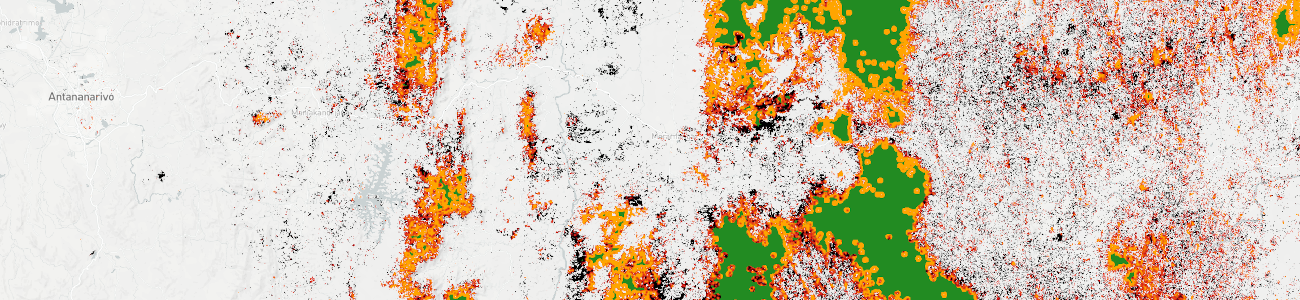
\includegraphics[width=10cm]{figs/riskmapjnr-example}\\
    \vspace{0.3cm}
    \small{Ghislain VIEILLEDENT$^{1}$\hspace{0.25cm}Pierrick RAMBAUD$^{2}$\hspace{0.25cm}Rémi d'ANNUNZIO$^{2}$}\\
    \vspace{0.15cm}
    {\scriptsize
      \begin{tabular}{l}
        $[1]$ \textbf{Cirad} UMR AMAP, $[2]$ \textbf{FAO} REDD$+$ NFM
      \end{tabular}
    }\\
    \vspace{0.3cm}
    
\includegraphics[width=0.75\textwidth]{figs/partners_logos}
    
  \end{center}
  \end{frame}
}

% %%%%%%%%%%%%%%%%%%%%%%%%%%%%%%%%%%%%%%%%%%%%%%%%%%%%%%%%%%%%%%%%

\placelogotrue
\begin{frame}
  \frametitle{Plan}
  \begin{columns}[c]
    \begin{column}{0.5\textwidth}
      \tableofcontents[sections=1]
      \vspace{0.5cm}
      \tableofcontents[sections=2]
    \end{column}
    \begin{column}{0.5\textwidth}
        \tableofcontents[sections=3]
        \vspace{0.5cm}
        \tableofcontents[sections=4]
    \end{column}
  \end{columns}
\end{frame}
\placelogofalse

\section{Introduction}
\label{sec:orged914c1}

\subsection{Context}
\label{sec:orge7f824b}

\begin{frame}[label={sec:orge78355b}]{Context}
\begin{itemize}
\item Paris Agreement on climate change
\item REDD+: Reducing Emissions from Deforestation and forest Degradation
\item IMPRESS (Improving Measurement for Payments to Reduce Emissions and Strengthen Sinks) FAO -- UK-PACT project
\item VCS Jurisdictional and Nested REDD+ (JNR): certification of jurisdictional REDD+ programs and nested projects
\end{itemize}

\begin{center}
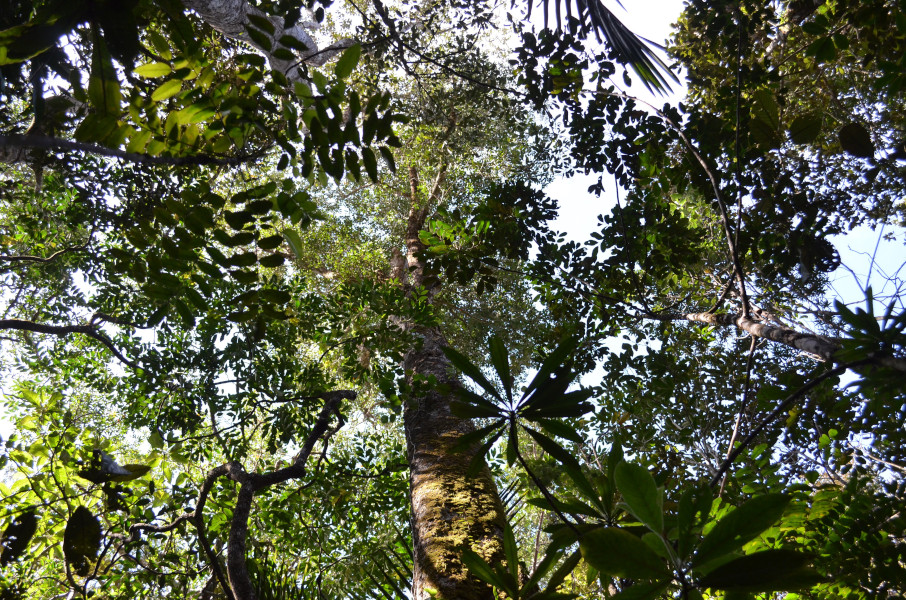
\includegraphics[width=0.5\textwidth]{figs/Canopy-NC.jpg}
\end{center}
\end{frame}

\subsection{Objectives}
\label{sec:org5a4da93}

\begin{frame}[label={sec:org79745ff}]{Objectives}
\begin{itemize}
\item Given a deforestation intensity (ha/yr), how to allocate deforestation \alert{spatially}? \(\Rightarrow\) Map of deforestation risk
\item Develop a tool to derive a map of the deforestation risk
\item Following JNR methodology
\item Using only an historical forest cover change map on a recent period
\end{itemize}

\begin{center}

\includegraphics[width=0.5\textwidth]{figs/jnr.png}
\end{center}
\end{frame}

\section{Functionalities}
\label{sec:orge5ec792}

\subsection{Python package}
\label{sec:orgb128efa}

\begin{frame}[label={sec:orgb67c257},fragile]{Python package and website}
 \begin{itemize}
\item Python package: \texttt{riskmapjnr}
\item Website: \url{https://ecology.ghislainv.fr/riskmapjnr}
\item GitHub repository with open source code: \url{https://github.com/ghislainv/riskmapjnr}
\item Tutorials: see \emph{Get Started} and \emph{Articles} sections on the website
\end{itemize}

\begin{figure}[htbp]
\centering
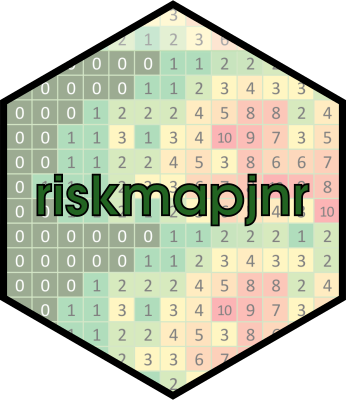
\includegraphics[width=0.25\textwidth]{figs/logo-riskmapjnr.png}
\caption{\texttt{riskmapjnr} logo}
\end{figure}
\end{frame}

\subsection{Functions}
\label{sec:org6a1ac31}

\begin{frame}[label={sec:org8002631},fragile]{Distance to forest edge threshold}
 \begin{itemize}
\item \texttt{rmj.dist\_edge\_threshold()}: Compute the distance to the forest edge after which the risk of deforestation becomes negligible.
\item Here, >99\% of deforestation occurs within a distance \(\le\)180m.
\item Forest pixels with a distance >180m will be in Category 0 (zero risk of deforestation).
\end{itemize}

\begin{figure}[htbp]
\centering
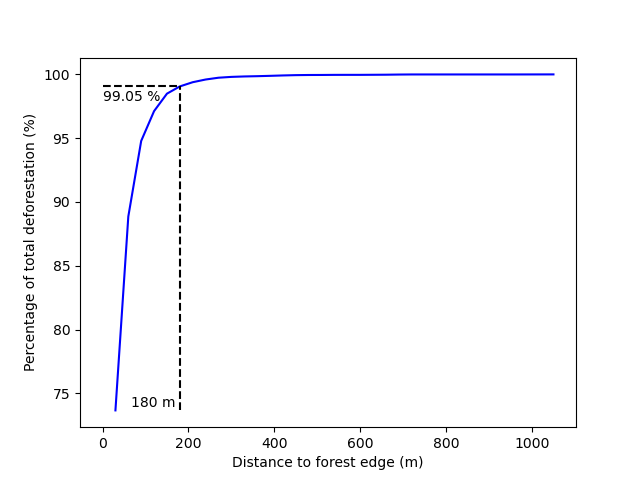
\includegraphics[width=0.5\textwidth]{figs/perc_dist.png}
\caption{\label{fig:org265194b}Cumulative deforestation as function of the distance to forest edge}
\end{figure}
\end{frame}

\begin{frame}[label={sec:org262743c},fragile]{Local deforestation rate}
 \begin{itemize}
\item \texttt{rmj.local\_defor\_rate()}: Compute a local risk of deforestation at the pixel level using a moving window made of several pixels.
\item Different window sizes can be chosen.
\item The JNR methodology recommends the use of 25 different window sizes.
\end{itemize}

\begin{figure}[htbp]
\centering
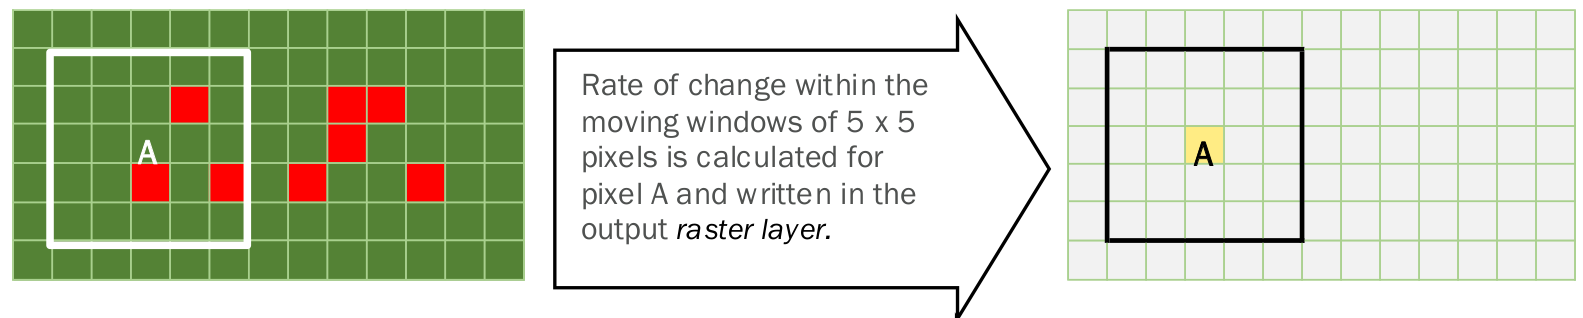
\includegraphics[width=0.8\textwidth]{figs/moving_window.png}
\caption{\label{fig:orgdd64615}Moving window}
\end{figure}
\end{frame}

\begin{frame}[label={sec:orgeceef08},fragile]{Categorize the deforestation risk}
 \begin{itemize}
\item \texttt{rmj.defor\_cat()}: Convert local deforestation rate into categories of deforestation risk.
\item The JNR methodology suggests to use \uline{31 categories of risk} from ``0'' to ``30'' (including the ``0'' category).
\item The JNR methodology recommends the use of \uline{three slicing algorithms}: ``equal area'', ``equal interval'', and ``natural breaks''.
\begin{itemize}
\item ``equal area'': each class covers approximately the same area
\item ``equal interval'': bins of the same range size
\item ``natural breaks'': data are normalized before applying the ``equal interval'' algorithm.
\end{itemize}
\end{itemize}

\begin{figure}[htbp]
\centering
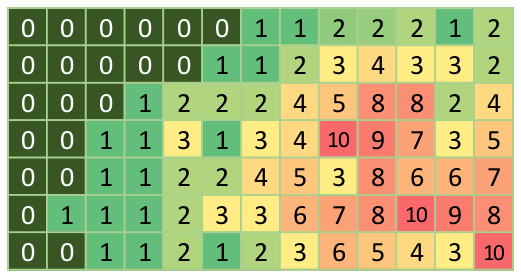
\includegraphics[width=0.4\textwidth]{figs/categories.png}
\caption{\label{fig:org719065e}Categories of deforestation risk}
\end{figure}  
\end{frame}

\section{Case-studies}
\label{sec:orgaf20642}

\subsection{Countries}
\label{sec:org68b9723}

\begin{frame}[label={sec:org969b8de}]{Countries}
\begin{columns}
\begin{column}{0.5\columnwidth}
\begin{itemize}
\item Guadeloupe (\emph{Get Started} tutorial)
\item Kenya (IMPRESS project)
\item Madagascar
\end{itemize}
\end{column}

\begin{column}{0.5\columnwidth}
\begin{figure}[htbp]
\centering
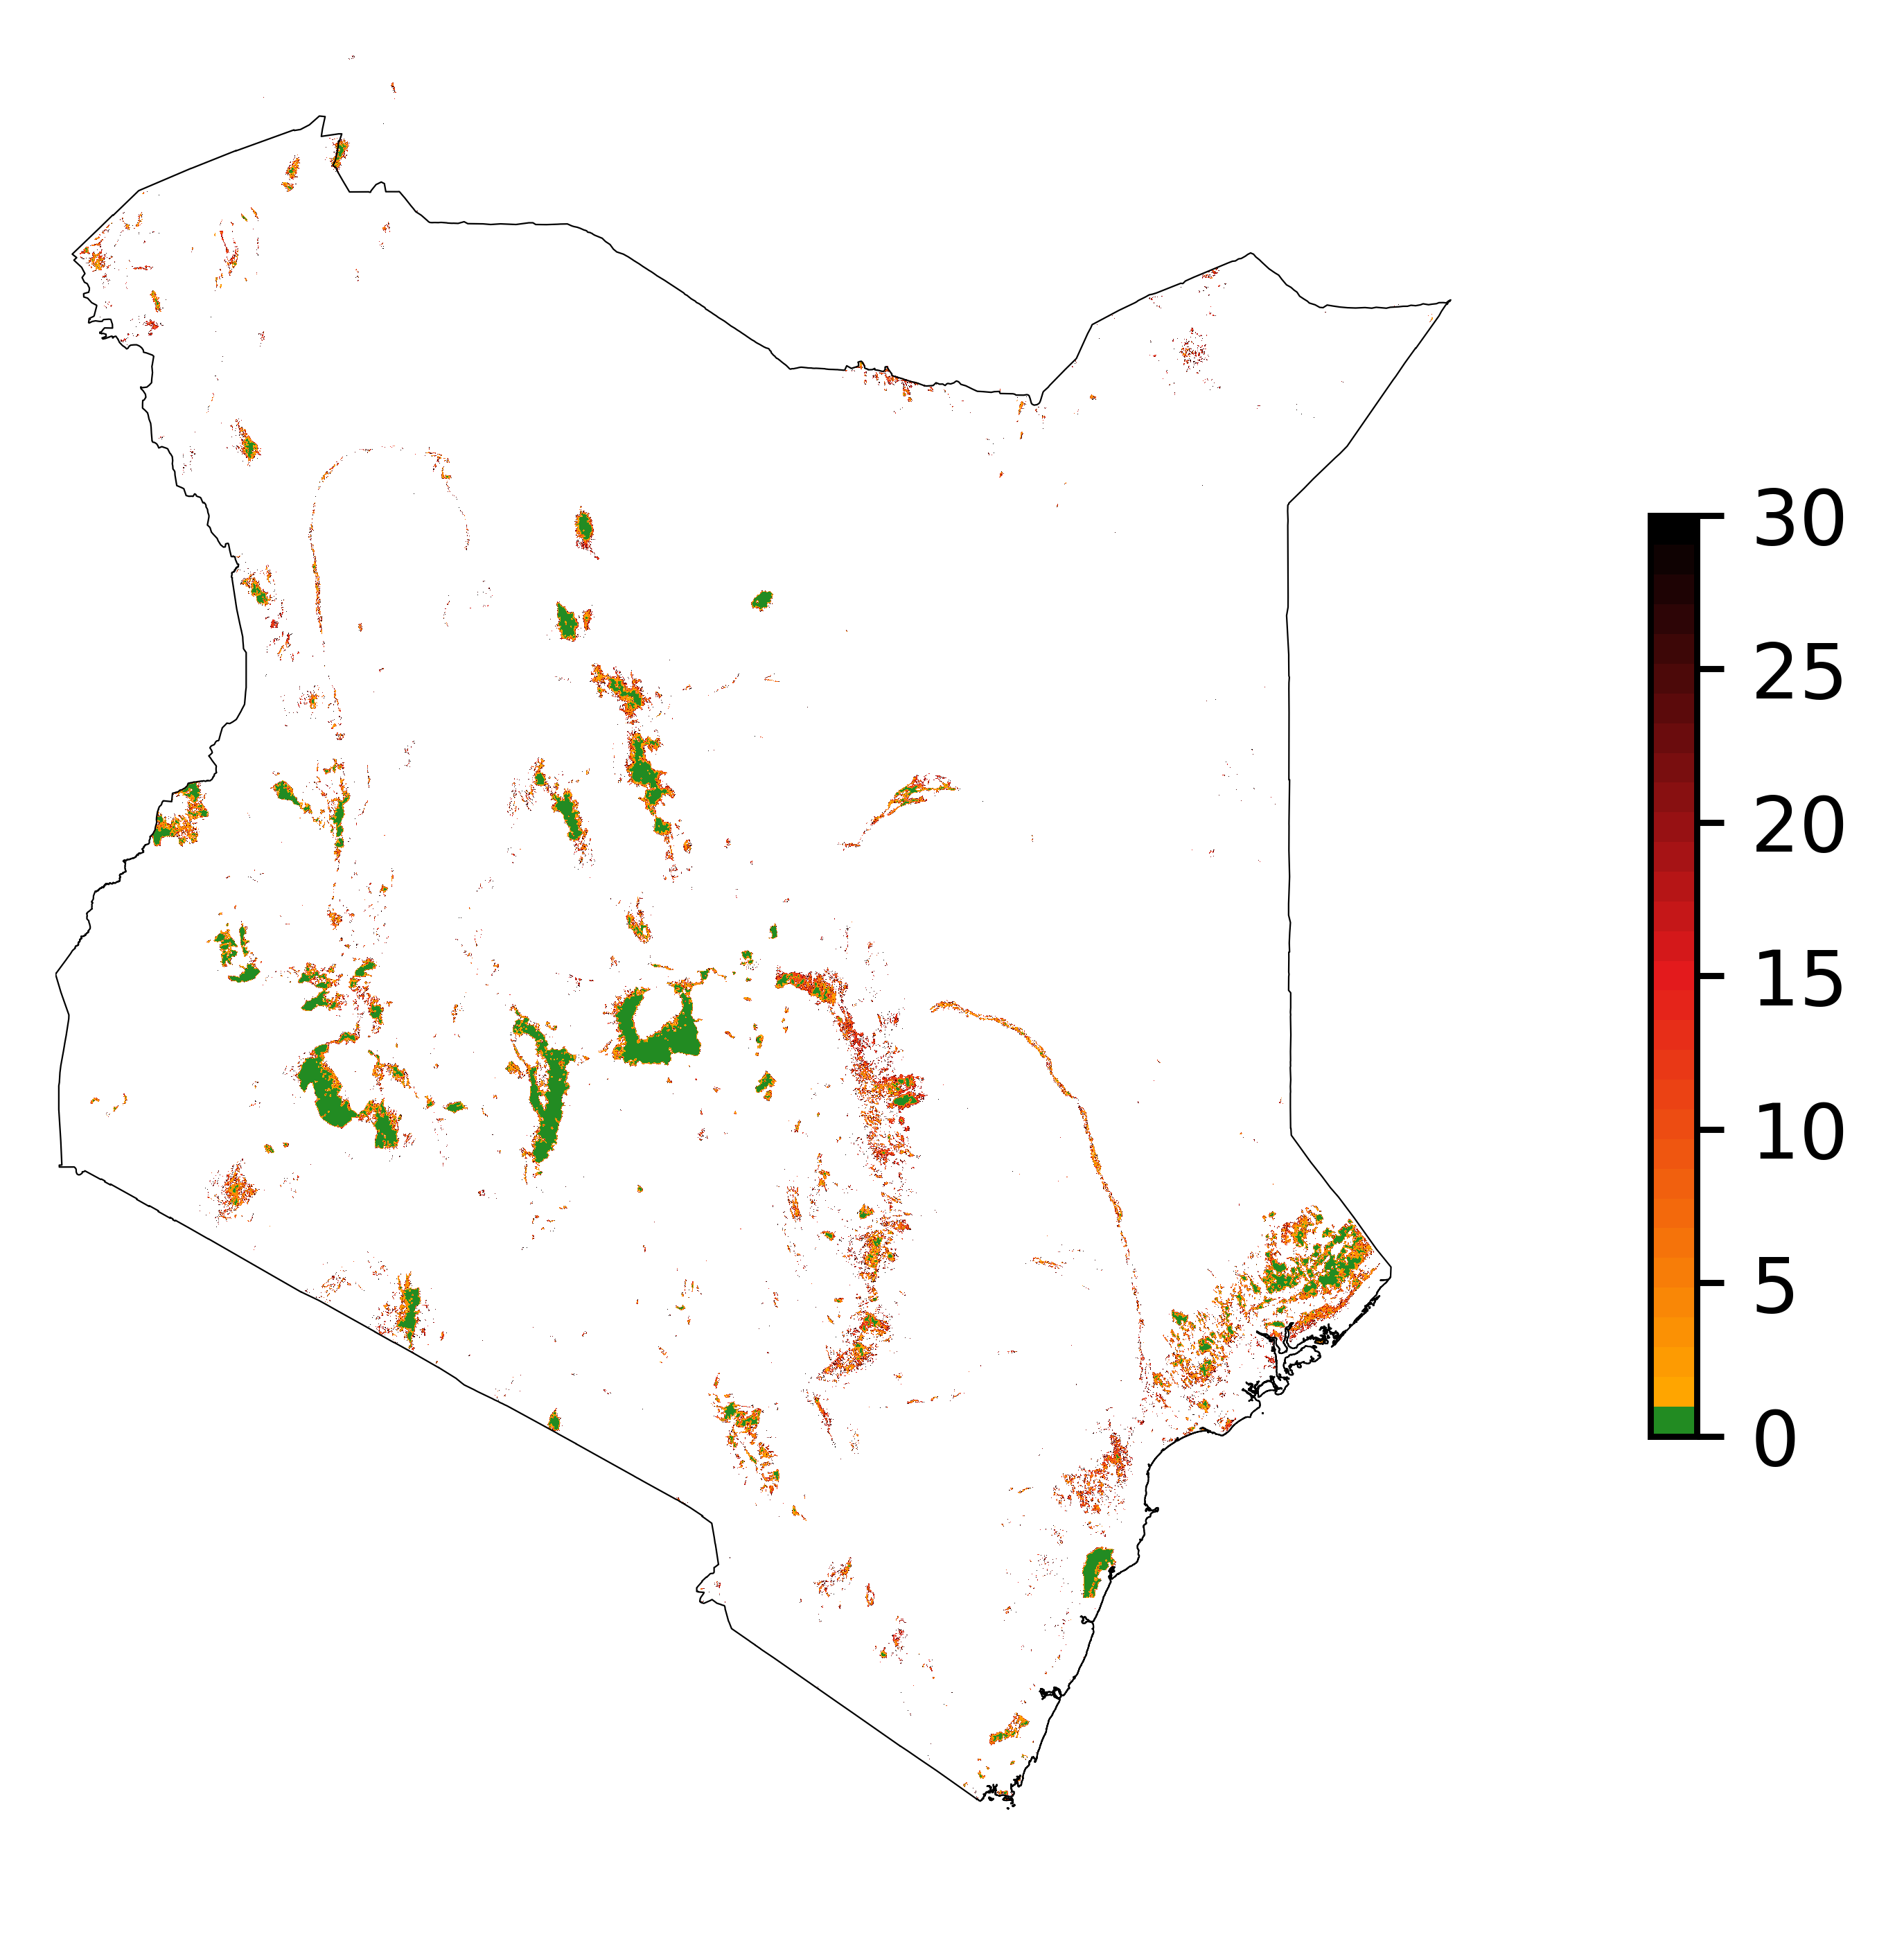
\includegraphics[width=\textwidth]{figs/riskmap_kenya.png}
\caption{\label{fig:orgf55086c}Map of deforestation risk for Kenya}
\end{figure}
\end{column}
\end{columns}
\end{frame}


\section{Perspectives}
\label{sec:org50d43e1}

\subsection{Comments}
\label{sec:org27f0b31}

\begin{frame}[label={sec:org770e38d}]{Additional tests}
\begin{itemize}
\item \alert{!!} First results
\item Code might include some errors
\item Functions still need to be thoroughly tested
\item Results must be consolidated
\end{itemize}
\end{frame}

\begin{frame}[label={sec:org86e3aea}]{Issues}
\begin{columns}
\begin{column}{0.5\columnwidth}
\begin{itemize}
\item The best window size is always the smallest
\item No differences between slicing algorithms (ei or ea)
\item ei: ``equal interval''\\
ea: ``equal area''
\end{itemize}
\end{column}

\begin{column}{0.5\columnwidth}
\begin{figure}[htbp]
\centering
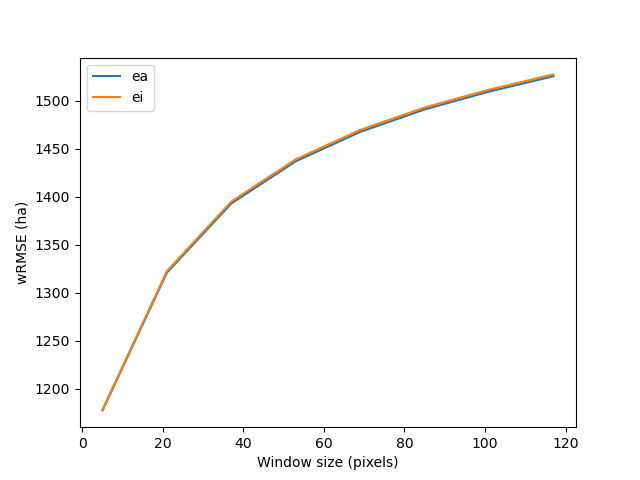
\includegraphics[width=\textwidth]{figs/map_comp.png}
\caption{\label{fig:org8ae83e2}Prediction error as a function of window size}
\end{figure}
\end{column}
\end{columns}
\end{frame}

\subsection{Alternative approach}
\label{sec:org7b5317d}

\begin{frame}[label={sec:org407cecd},fragile]{Comparison with the \texttt{forestatrisk} approach}
 \begin{itemize}
\item Alternative approach to compute the deforestation risk
\item Statistical model estimating the deforestation risk \(\theta\)
\item \(\theta\) = function(environmental variables + location)
\item Variables: distance to forest edge, roads, towns, protected areas
\end{itemize}
\end{frame}

% %%%%%%%%%%%%%%%%%%%%%%%%%%%%%%%%%%%%%%%%%%%%%%%%%%%%%%%%%%

{
  % Use background image
  \usebackgroundtemplate{%
    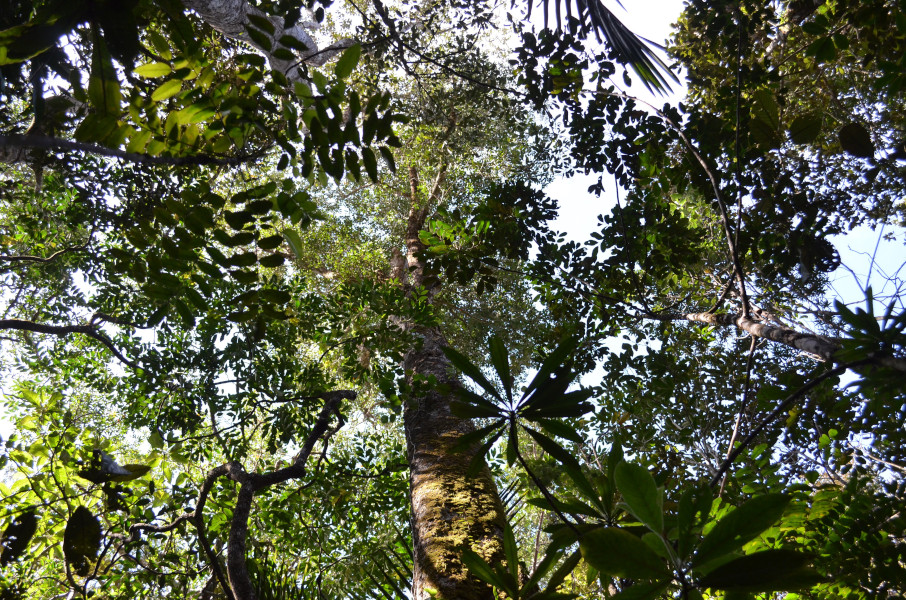
\includegraphics[keepaspectratio=true, height=\paperheight]{figs/Canopy-NC}
  }
  \setbeamertemplate{navigation symbols}{}
  % Remove shadow from block
  \setbeamertemplate{blocks}[rounded][shadow=false]
  \begin{frame}[plain]
  	\vspace*{\stretch{100}} 
    \begin{block}{}
      \begin{center}
        \ldots~Thank you for attention~\ldots \\
        \url{https://ecology.ghislainv.fr/presentations} \\
        
\includegraphics[width=0.45\textwidth]{figs/partners_logos}
      \end{center}
    \end{block}
  \end{frame}
}
\end{document}